%!TEX root = kotov.tex
\section{Task 5}
\begin{task}
    Докажите, что для поиска максимума в массиве различных чисел потребуется как минимум $n - 1$ сравнение.
\end{task}

\begin{solution}
    Какое-то очень коротенькое док-во (скорее показательство): рассмотрим задачу нахождения максимума, как турнир среди $n$ участников, где в ``дуэли'' побеждает больший из пары. Тогда, чтобы определился победитель турнира (то есть нашелся максимум), надо, чтобы остальные участники проиграли как минимум один раз, а таких участников $n-1$ штука.
    \begin{figure}[H]
        \centering
        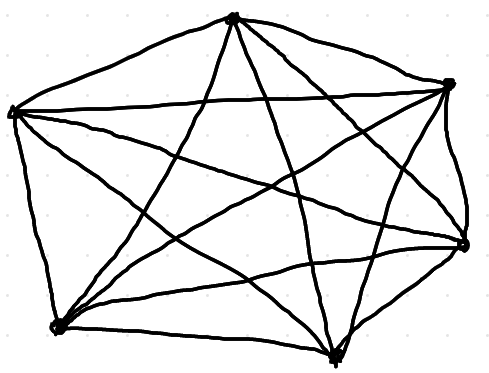
\includegraphics[scale=0.3]{pics/5.png}
        \caption{Турнир, а не пентаграмма (к тому же вершин 6), забыл стрелочки нарисовать :с}
    \end{figure}
\end{solution}

\begin{solution}
    (Второй способ ?) Посмотрим на случай $n = 2$. Очевидно, чтобы понять кто больше, нам необходимо сделать ровно одно сравнение. Пусть, не умаляя общности, $x_1 < x_2$ и заведем $x_{\text{max}} = x_2$. Что происходит, когда к нам приходит еще один эл-т $x_3$? Нам надо понять, может ли он быть новым наибольшим элементом? Для этого достаточно провести одно сравнение с $x_{\text{max}}$, то есть итого на данном этапе у нас проведено $1+1$ сравнение. Если $x_2 < x_3$, то заменим $x_{\text{max}}$ пришедшим эл-том,если же $x_2 \geq x_3$, то просто выбросим $x_3$ и продолжим ``получать'' новые элементы. С каждым новым элементом мы будем проводит одно сравнение, то есть $\texttt{cnt} +\!\!= 1$, а изначально, на первом шаге, $\texttt{cnt} = 1$. Таким образом, когда мы расширим количество элементов до $n$ мы проведем $1 + (n-2) = n-1$ сравнений, чтобы выяснить кто же является наибольшим.
\end{solution}